\chapter{Identifying significant parameters combinations in complex
  models \label{ch:params}}


% \begin{abstract}
%   Detailed dynamical models can often be summarized in terms of only
%   a few components, reducing complexity and making exploration
%   easier and more insightful.  Pen-and-paper reduction is tedious
%   and impractical for most models, however it has the added benefit
%   of identifying parameter combinations that matter most.  Recently
%   developed frameworks computerizing model reduction leave the dual
%   aspect of effective parameter identification unaddressed,
%   relegating parameter space exploration subject to ineffective
%   sampling strategies.  Here, we lay the foundation for systematic
%   parameter reduction, rooting it in the same nonlinear data mining
%   techniques that powered model reduction in our earlier
%   equation-free framework.  Our ambition is to extend the
%   data-driven determination of effective variables by integrating
%   into it the discovery of effective model parameters.  This will
%   accelerate both dynamical simulations and parametric explorations,
%   allowing us to efficiently map out the behavior of complex models.

% \end{abstract}

The past decades have seen a steady fall in the cost of computation,
enabling systems to be studied using increasingly complex models.
Perceptron networks in the 1960's contained thousands of hidden units
\cite{nagy_neural_1991}, while modern neural nets are
comprised of billions \cite{hsu_biggest_2015}. Molecular dynamics simulations in 1957 entailed tens of
hard-sphere particles \cite{alder_phase_1957}; today we model entire proteins and their folding dynamics
\cite{piana_atomic-level_2013}. And Lorenz's
three-dimensional system of equations describing atmospheric
convections in 1963 \cite{lorenz_deterministic_1963} led to
modern large eddy simulations run across multiple computing clusters
\cite{ghosal_dynamic_1995}. In all cases, the improvement in precision
afforded by increased model complexity is matched by an increased
number of model parameters.

Highly parameterized models may aid accuracy, but the effect of each
individual parameter on the overall model output is often difficult to
ascertain. Indeed, it has been well-document that a wide array of
systems contain particular hidden parameters that appear to have no
influence on the model's predictions. These have been termed ``sloppy
parameters'', and their presence seems ubiquitous in contemporary
systems \cite{gutenkunst_extracting_2007}. This is problematic as not only do sloppy parameters
obfuscate the parameters that actually matter, but they also lead to
slow convergence of model-fitting algorithms \cite{transtrum_geometry_2011}.

Several approaches have been suggested to combat this
over-parameterization. Some, such as the Manifold Boundary
Approximation Method ultimately rely on deriving by hand a reduced
model \cite{transtrum_model_2014}. Others, such as
Active Subspaces make assumptions about linearity that may not hold in
practical settings \cite{constantine_active_2015}. Here, we present a
data-driven approach to parameter reduction that is flexible enough to
handle nonlinear systems. This is accomplished through Diffusion Maps
(DMAPS), an established manifold learning technique that we adapt to
the problem at hand \cite{coifman_diffusion_2006}. We begin with a description
of our broader view of the situation, and then present a simple
example that clearly shows the consequences of sloppiness, while also
providing some intuition as to how it emerges.

Our overall approach to this problem is motivated by the work in
\cite{transtrum_geometry_2011}. We consider a model to consist of a vector
of parameters $\theta \in \mathbb{R}^k$ and a function mapping these
inputs to a model response, or output, in $\mathbb{R}^n$,
$f: \mathbb{R}^k \rightarrow \mathbb{R}^n$. Sloppiness would reveal
itself as regions of parameter space, $\Omega_S \in \mathbb{R}^k$ in
which the model reponse remains nearly constant:
$f(\theta_i) \approx f(\theta_j)\; \theta_i, \theta_j \in
\Omega_S$. We will also denote distances in model response space as
$\delta(\theta_i, \theta_j) = \| f(\theta_i), f(\theta_j)\|_2$. To
provide a concrete example, consider a model with parameters $p_1$ and
$p_2$, and model output
$f(p_1, p_2) = (p_1 p_2 , \ln(p_1) + \ln(p_2) , (p_1 p_2)^2)$. Then
$\theta = (p_1, p_2) \in \mathbb{R}^2$ and $f: \R^2 \rightarrow
\R^3$. It is clear from the expression for $f$ that the model response
depends only on the overall product $p_1 p_2$, and not on $p_1$ and
$p_2$ independently. To make it explicit, set $p_{eff} = p_1 p_2$ and
rewrite $f$ as $(p_{eff}, \ln(p_{eff}), p_{eff}^2)$. Thus, although we
have chosen to include both $p_1$ and $p_2$ as independent parameters
in our original model, only the value of $p_{eff}$ matters. Also note
that if we only had access to a black-box function evaluator, it would
be non-trivial to determine the existence of $p_{eff}$ at all.

This model is illustrated in Figure~\ref{fig:non-id}, where curves of
constant color denote sets of constant model response. If we had
sampled data corresponding to true parameter values of
$p_1^* = p_2^* = 1$, Figure~\ref{fig:non-id} also reveals how
sloppiness affects optimization routines trying to fit such
data. Convergence is permitted along entire bands of parameter space
instead of at a single point. The inset shows $\delta$-contours of a
slightly perturbed system in which both $p_1$ and $p_2$ influence $f$;
however, certain directions, namely along the diagonal, still affect
model output more strongly than others. In addition, optimization
routines will still converge to disparate points in the plane: the
model remains sloppy. 

Our goal, then, is to extract the approprate, intrinsic
parameterization of the model using only input-output data. As we
shall see, this parameterization may vary across input space regimes.
We will show how this variation can be associated with the traditional
notions of regular and singular perturbations in explicit models when
the number of effective parameters changes.


\begin{figure}
  \centerline{\includegraphics[width=1.0\linewidth]{p2-p1-delta}}
  \caption[Illustration of effects of sloppiness on
  optimization]{Coloring the $(p_1, p_2)$ plane by $\delta$ for
    $f(\theta) = (p_1 p_2 , \ln(p_1) + \ln(p_2) , (p_1 p_2)^2)$ (main
    figure) and the perturbed $g(p1, p2) = f(p_1, p_2) +
    \left(2*\epsilon*(p1 - p2), 0, 0\right)$ with $\epsilon = 0.2$
    (inset). $\delta$ values are calculated with respect to the base
    parameters $p^* = (1, 1)$: $\delta(p_1, p_2) = \| f(p_1, p_2) -
    f(p_1^*, p_2^*)\|$. Also shown are a range of initial and final values of
    a gradient descent algorithm. For $f$, convergence can occur
    anywhere along the infinite band for which $\delta$ is less than
    the accepted tolerance. For $g$, convergence is confined to
    bounded but stretched regions in the plane.
    \label{fig:non-id} }
\end{figure}



\subsection{Unraveling sloppiness} \label{sec:rr} 

We now examine a system of chemical reactions in which an effective
parameter again emerges, and show how we can detect this in a
data-driven manner. The three-species system is

\begin{align}
  A
  \xrightleftharpoons[k_{-1}]{k_1}
  B
  \xrightarrow[]{k_2}
  C
  \label{mech:abc}
\end{align}

Under mass action kinetics, the concentration of the end product is
given by the analytical expression
% 
\begin{align}
  C(t|\theta)
  =
  A_0
  \left(
  \frac{k_1 k_2}{\alpha \beta}
  +
  \frac{k_1 k_2}{\alpha(\alpha - \beta)}
  e^{-\alpha t}
  -
  \frac{k_1 k_2}{\beta(\alpha - \beta)}
  e^{-\beta t}
  \right)
  \label{eq:cfull}
\end{align}
% 
where $(A_0,B_0,C_0)$ are the fixed constituent concentrations at time
zero and $\alpha,\beta$ depend on $\theta=(k_{-1},k_1,k_2)$; see
Appendix~\ref{app:abc} for the derivation. In the parameter regime
$k_1 k_2 \ll (k_1 + k_{-1} + k_2)^2$, \eqref{eq:cfull} is well
approximated by
% 
\begin{align}
  C_{eff}(t|\theta)
  =
  A_0
  \left(
  1 - e^{-k_{eff} t}
  \right) ,
  \quad
  k_{eff}
  =
  \frac{k_1 k_2}{k_{-1} + k_1 + k_2} .
  \label{ABC-QSSA}
\end{align}
% 
Note that this approximate solution extends to a larger parameter
range the quasi-steady state approximation (QSSA)
$C_\mathrm{QSSA}(t|\theta) = A_0 (1 - e^{-k_\mathrm{QSSA} t})$,
valid for $k_1 \ll k_{-1} + k_2$ with
$k_\mathrm{QSSA}=k_1 k_2/(k_{-1} + k_2)$.  Plainly, this approximate
solution represents an effective reduction of parameter space down to
the single parameter $k_{eff}$, the levels sets of which
foliate parameter space as in Fig.~\ref{fig:abc-ill}.

To verify that $C(t)$ remains roughly constant on these level sets, we
choose reference parameter settings $\theta^*$ in the regime
identified above, fix sampling times $t_1,\ldots,t_N$, set the model
response to $f(\theta)=( C(t_1|\theta) , \ldots , C(t_N|\theta) )$,
sample log-parameter space uniformly, and record the squared Euclidean
distance $\delta(\theta) = \| f(\theta) - f^* \|^2$ for each sampled
$\theta$.  Figure~\ref{fig:abc-keff} shows the results colored by
$k_{eff}$. We only retained parameter combinations with
$\delta(\theta) < 10^{-6}$ to aid in visualization. As expected, the
level sets of constant $\delta$ align with those of the effective
parameter, so this automated sampling process effectively reveals
sheets of the foliation in Fig.~\ref{fig:abc-ill} without recourse to
an analytic expression for $k_{eff}$.

\begin{figure}[!htp]
\centering
  \includegraphics[width=0.9\textwidth]{keff-illustration}
\caption[Illustration of level sets of the effective parameter in a
  model of chemical kinetics]{Illustration of level sets of $k_{eff}$ in parameter space. \label{fig:abc-ill}} 
\end{figure}


\begin{figure}[ht!]
  \centering
  \includegraphics[width=0.9\textwidth]{keffs-delta-keff-vertical}
  \caption[Quantitative three-dimensional views of level sets of the
  effective parameter in a model of chemical kinetics]{(top) Region of
    parameter space lying within large value of $\delta = 10^{-3}$,
    colored by $k_{eff}$. Smaller rotations show three-dimensional
    structure. (bottom) Plot of $\delta$ vs $k_{eff}$ over the dataset
    showing that $\delta(k_1, k_{-1}, k_2) = \delta(k_{eff})$ as
    expected from the reduced reaction kinetics. \label{fig:abc-keff}}
\end{figure}


\begin{figure}[!htp]
\centering
\begin{tabular}{cc}
  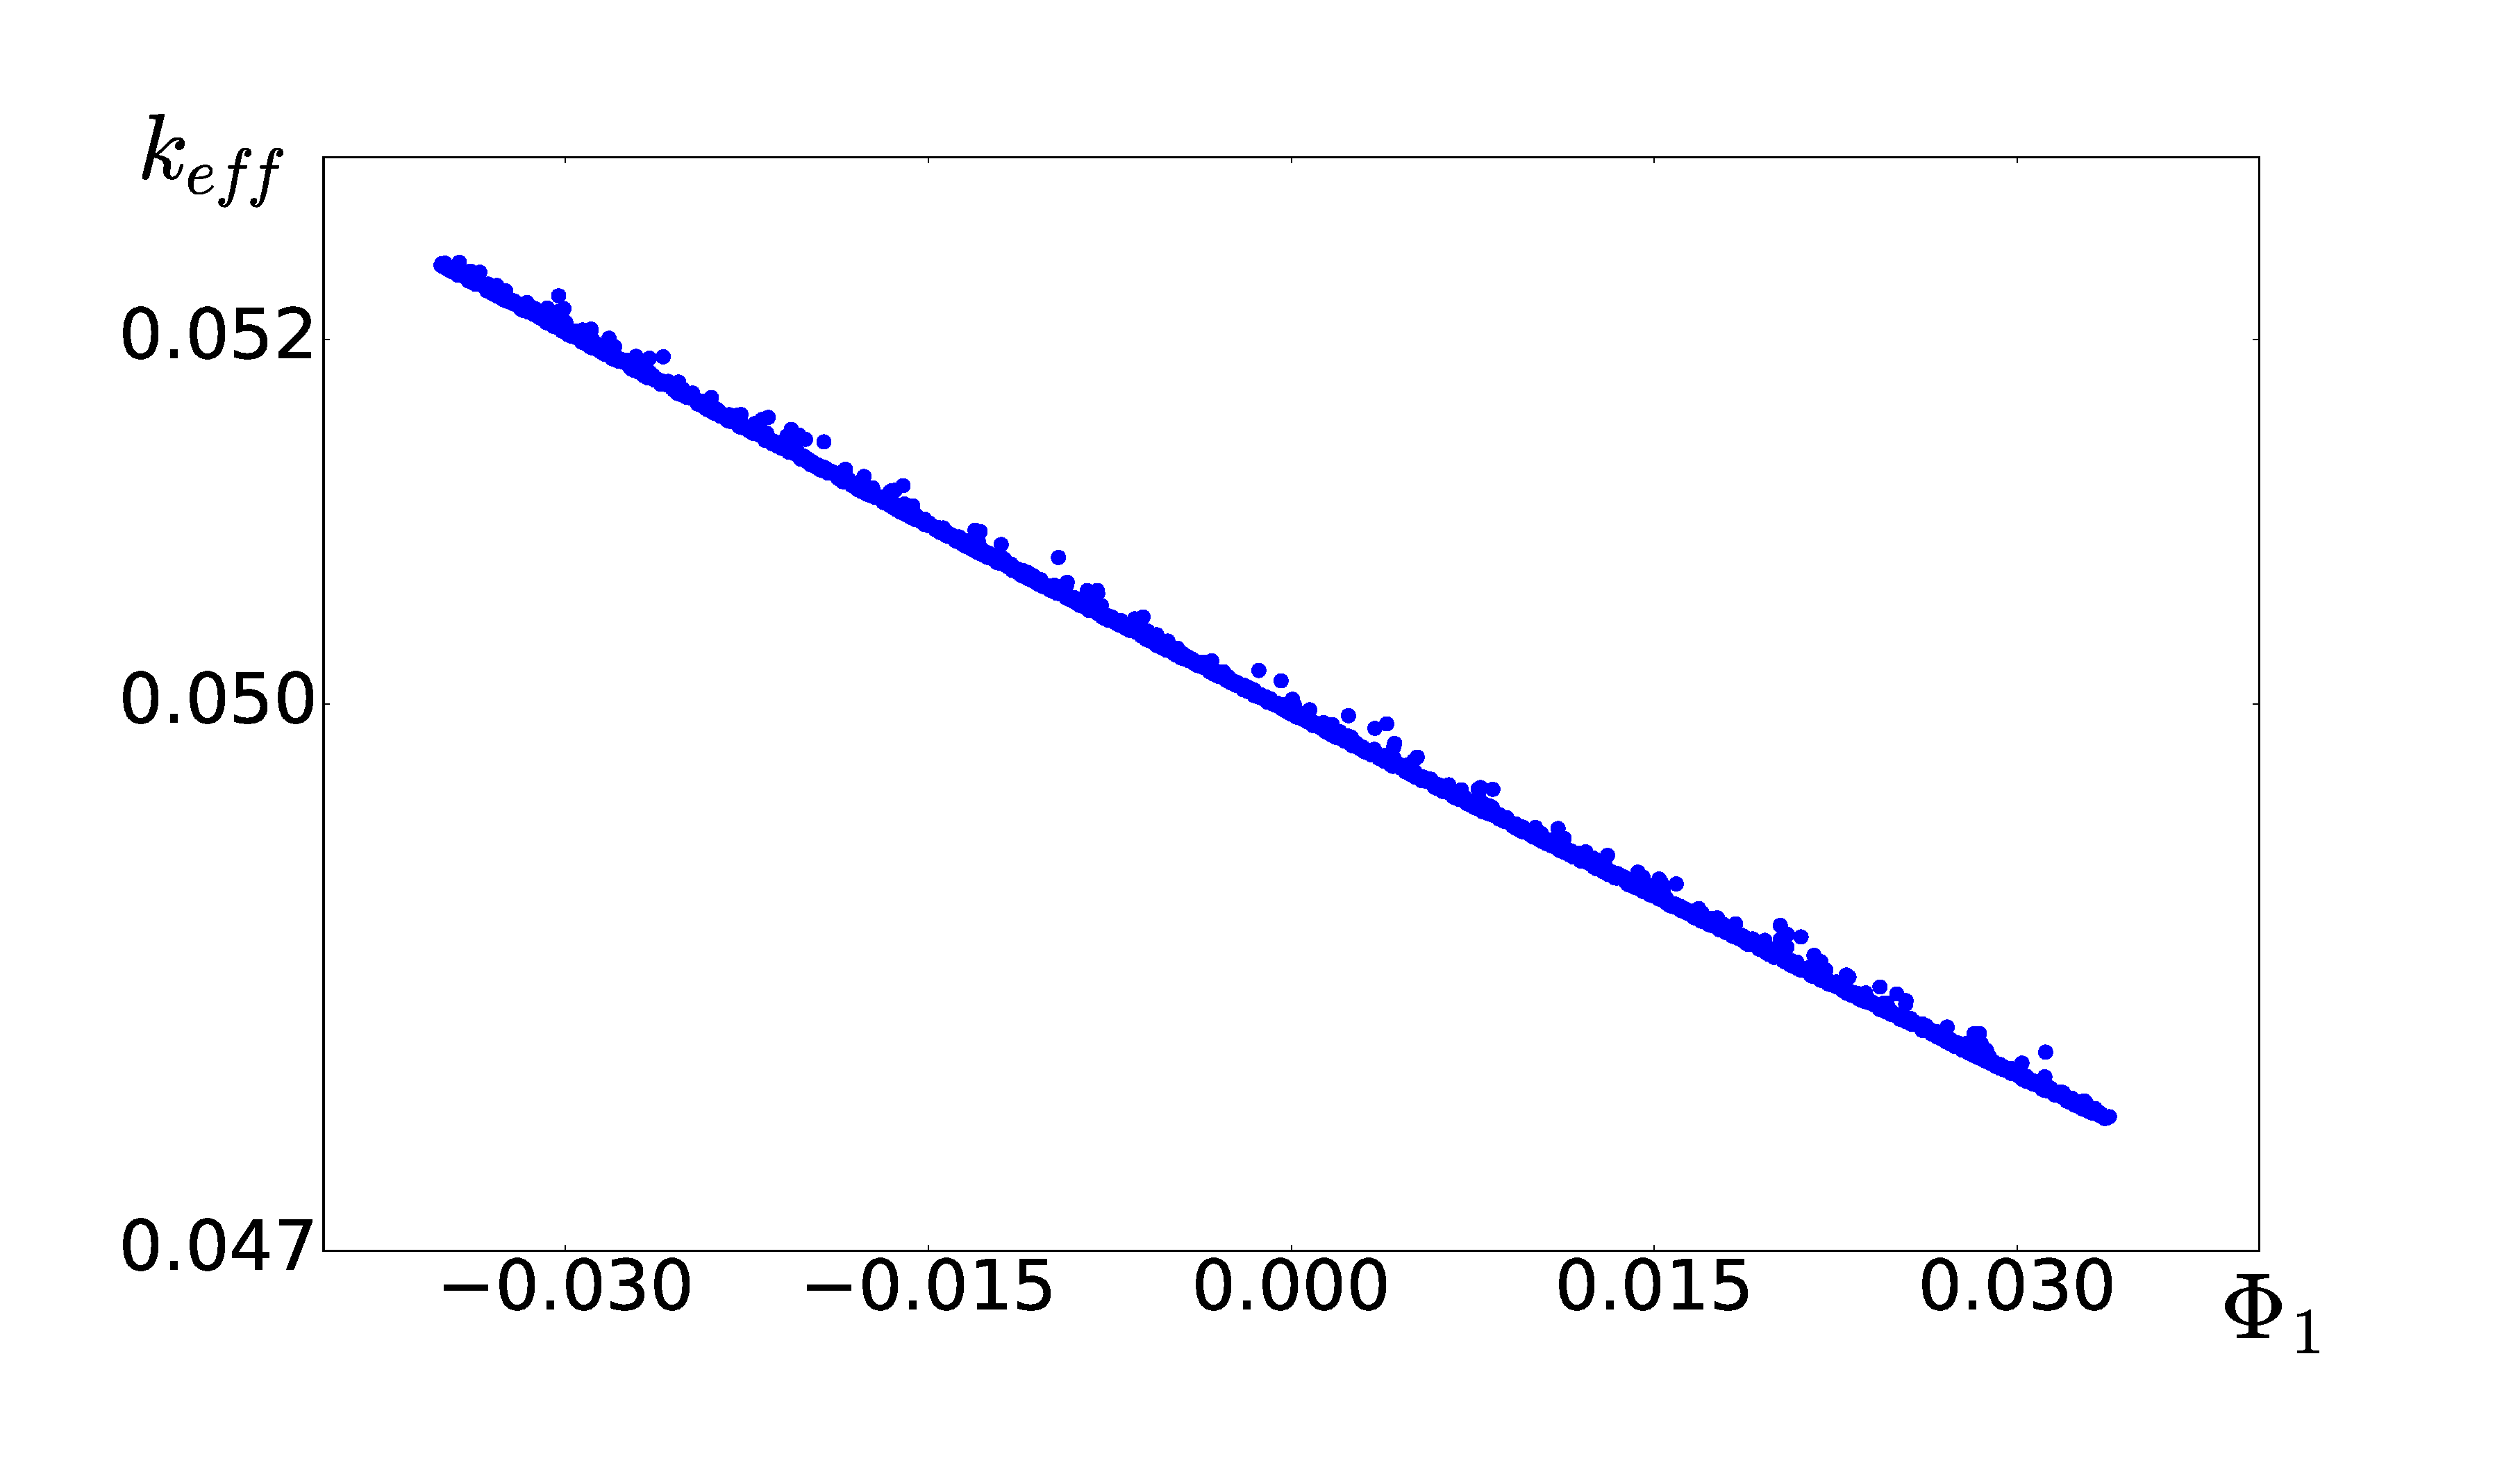
\includegraphics[width=0.45\textwidth]{keff-phi1} &
  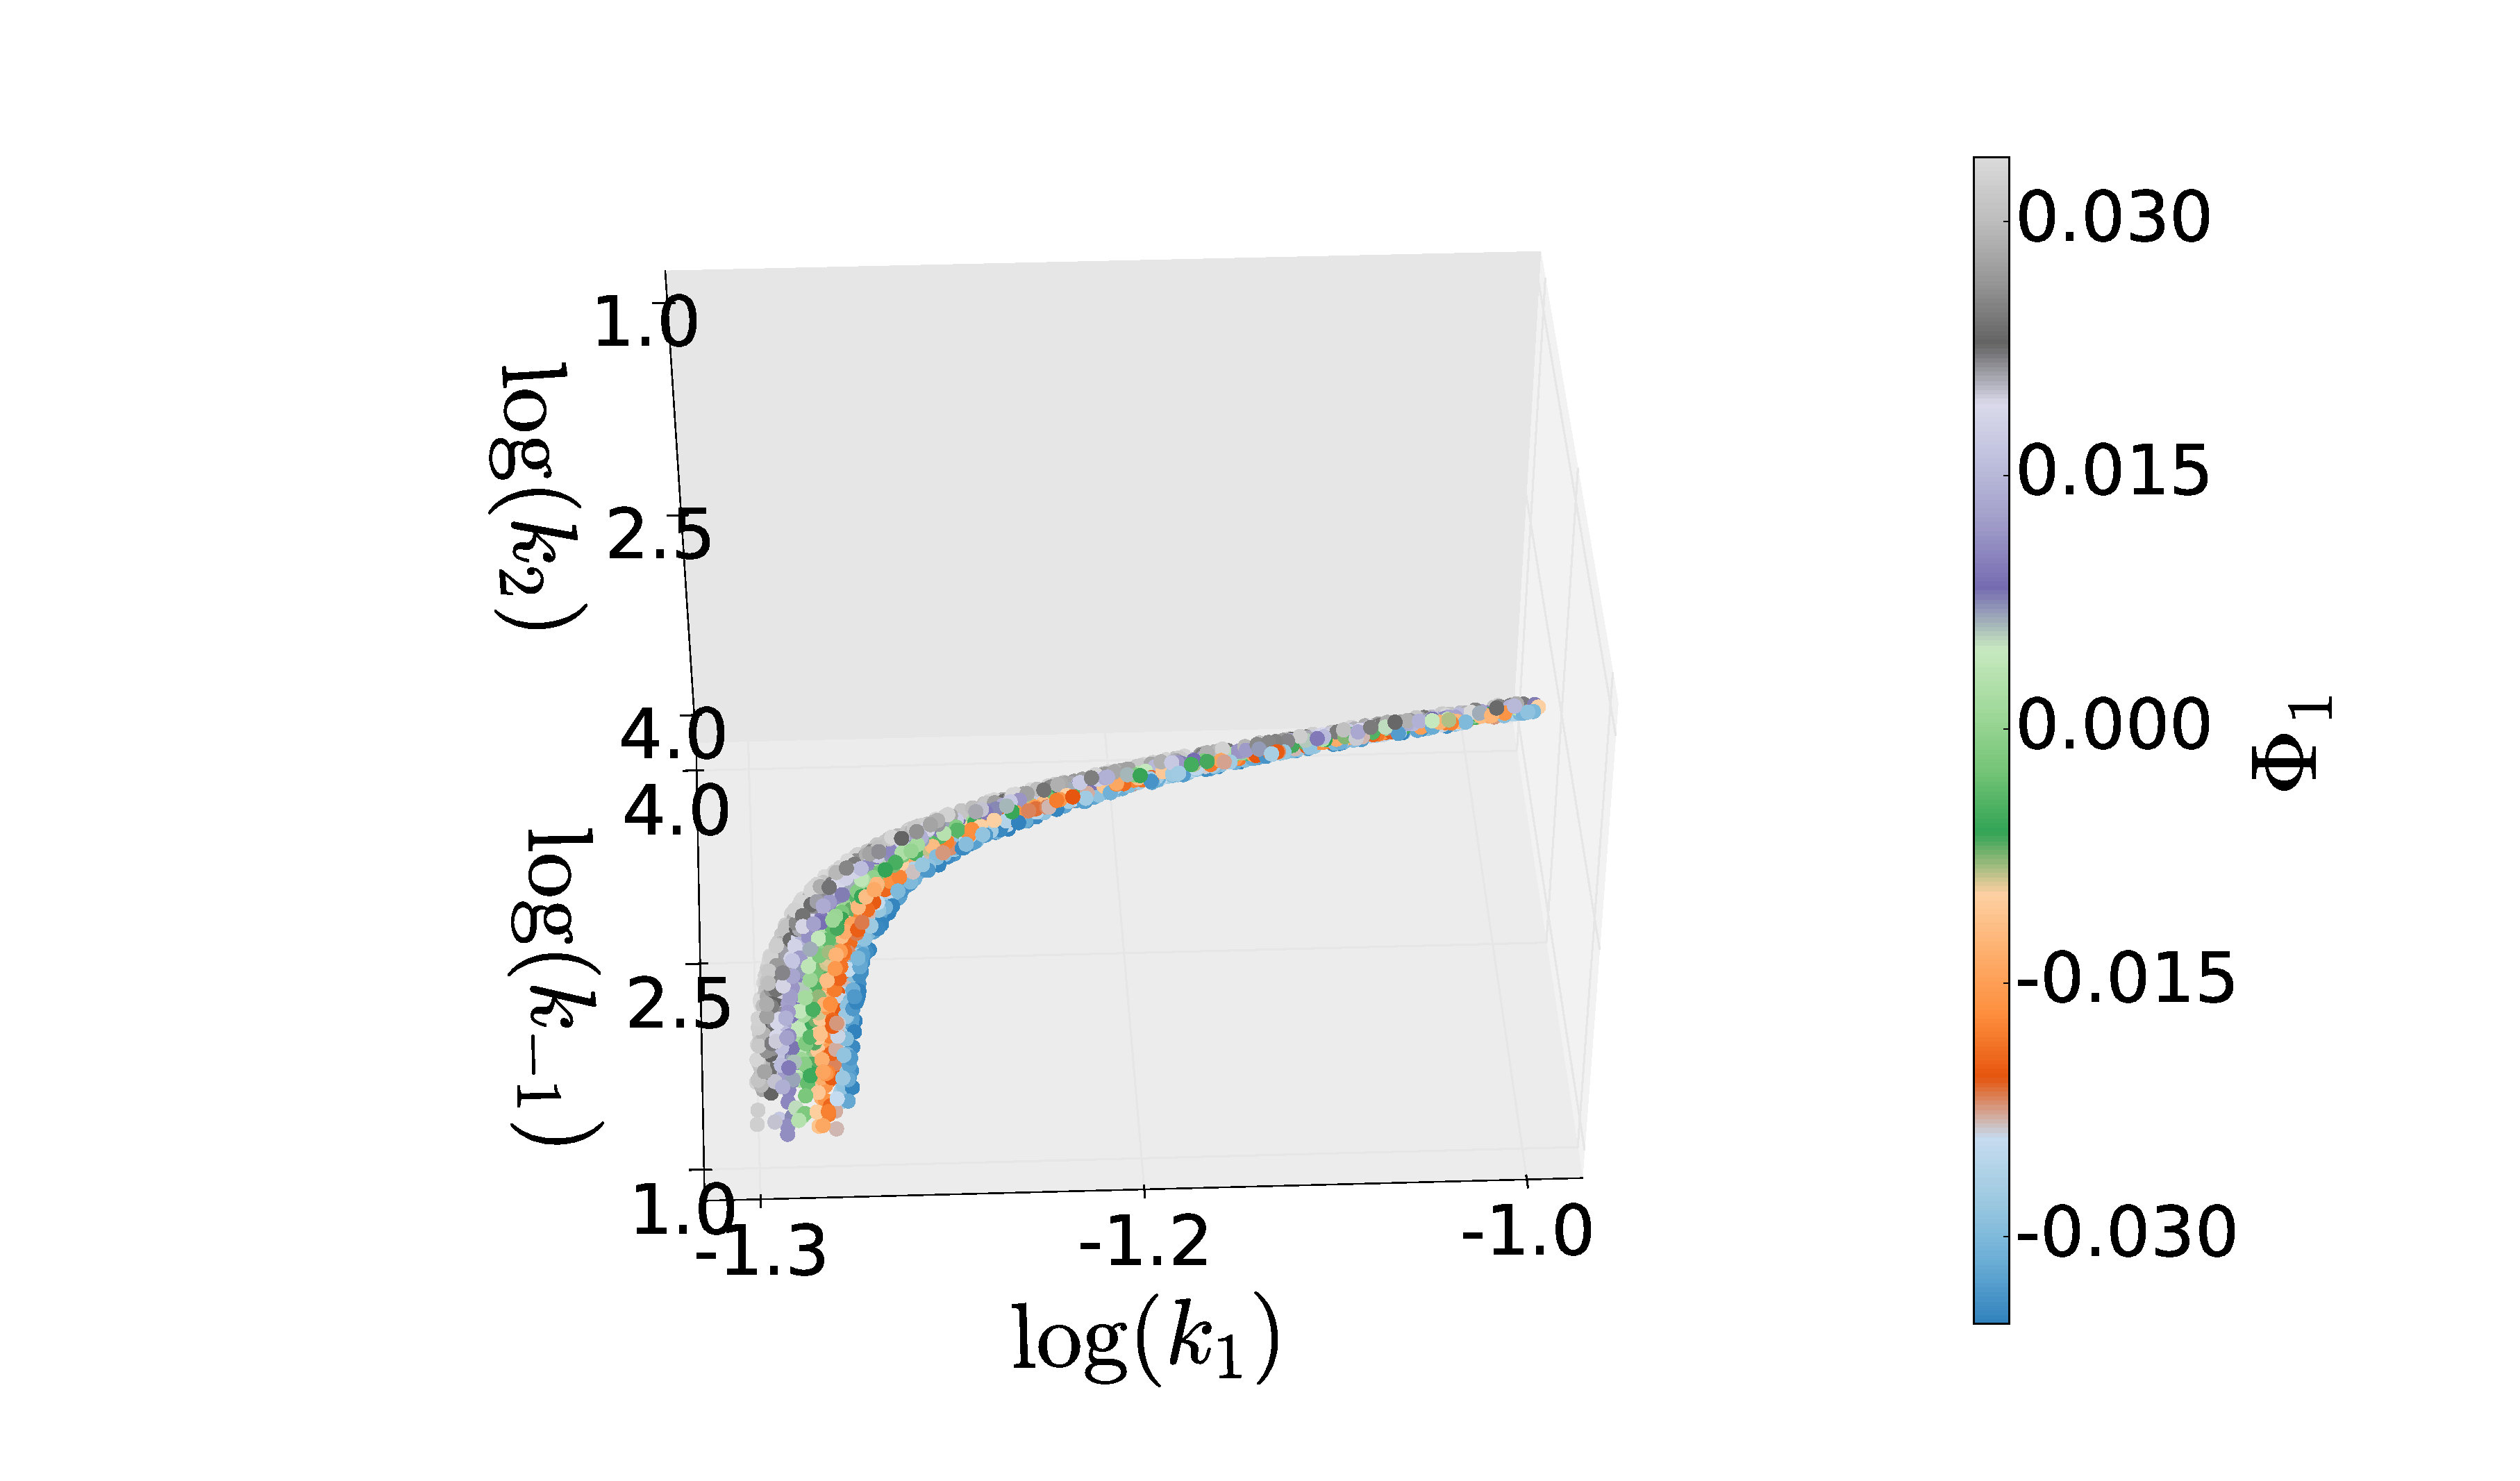
\includegraphics[width=0.45\textwidth]{k2-kinv-k1-phi1}\\
  (a) & (b)
\end{tabular}
\caption{(a) Coloring parameter space by $\phi_1$, showing that
  $\phi_1$ captures the effective parameter in this system; (b)
  $k_{eff}$ plotted against $\phi_1$ showing that the first DMAPS
  eigenvector parameterizes the significant, nonlinear parameter
  combination hidden in our model. \label{fig:abc-dmaps}} 
\end{figure}


With this data in hand, we turn to a description of our modified the
DMAPS algorithm. Details of the basic algorithm can be found in
Section~\ref{sec:dmaps}. In brief, given a collection of parameter
values ${\theta_i}_{i=1}^N$, we define our DMAPS kernel as

\begin{align}
  k(\theta_i, \theta_j) = \exp \left(-\frac{\|f(theta_i) -
  f(theta_j)\|^2}{\epsilon^2} \right)
  \label{eq:dmaps-mm}
\end{align}

The key point is that while the data in Figure~\ref{fig:abc-keff}
obviously represent a sample of parameter space, they simultaneously
sample the model response space through $f(\theta)$. Considering the
structure of this space, we can understand that all of the points
lying on a surface of constant $k_{eff}$ will be mapped to
approximately the same point in model response space. Only changes in
$k_{eff}$ affect the model output, and thus our data will lie along a
one-dimensional curve in model response space, parameterized by
$k_{eff}$. Therefore, if we apply DMAPS to the model response data,
the first eigenvector $\phi_1$ will likewise yield a parameterization
of this curve. Thus, we expect $k_{eff}$ and $\phi_1$ to be in
one-to-one correspondence. This is precisely what
Figures~\ref{fig:abc-dmaps} show DMAPS has, in effect, uncovered the
effective parameter hidden in the system using only paramter and model
response data. We will now investigate how sloppiness can arise in
singularly- and regularly-perturbed systems, and we will see that
DMAPS is able to detect these perturbed regimes.


\section{Regular perturbation}

Let us now consider the differential equation
%
\begin{equation}
 \frac{dy}{dt} = \epsilon y^3 - y
\quad
 y(0) = y_0 ,
\label{1D-model-regpert}
\end{equation}
%
with $\theta = (y_0, \epsilon)$ and $f(\theta) = \left(y(t_1), y(t_2), \dots,
  y(t_n) \right)$.

Unlike the previous two examples, there is no effective parameter
hidden in this system; however, our parameters affect the model output
very differently depending on their specific values. To see why this
is, consider what happens as $\eps \rightarrow 0$. The system becomes
regularly perturbed, and converges to the simpler
$\frac{dy}{dt} = -y$. Note that in this limit, $\eps$ has no influence
on the model response, and $y_0$ becomes the only significant
parameter. Again, considering the implications for the model manifold,
it is clear that for small values of epsilon, our response will form a
one dimensional curve parameterized by $y_0$. At larger values, both
$\eps$ and $y_0$ are significant, and the manifold is
two-dimensional. Figure~\ref{fig:regpert} (a) depicts the model
manifold colored by $\eps$, and we see exactly this behavior. The red
portion of the surface, corresponding to larger $\eps$ is
two-dimensional, while the blue, with small $\eps$, is contained in a
single line at the edge of the surface. Sampling this manifold, as
detailed in Appendix~\ref{app:regpert}, and applying DMAPS with the
kernel presented in Equation~\ref{eq:dmaps-mm} yields the same
information directly from data. Figure~\ref{fig:regpert} (b) shows the
$(\eps, y_0)$ parameter plane colored by $\phi_1$. At larger values of
$\eps$ the colors vary without any significant trend as this region is
two-dimensional. However, at small $\eps$, the colors flatten out
horizontally: $\phi_1$ is constant along lines of constant
$y_0$. DMAPS captures the fact that only one direction in parameter
space is relevant in the regularly perturbed regime. To continue along
this line in a slightly more complicated scenario, our next system
will be singularly perturbed.

\begin{figure}[ht!]
\centering
\begin{tabular}{cc}
\includegraphics[width=0.45\textwidth]{y3-y2-y1-eps} &
\includegraphics[width=0.45\textwidth]{y0-eps-phi1} \\
(a) & (b)\\
\end{tabular}
\caption{(a) Model manifold of regularly perturbed system with
  parameters $y_0$ and $\epsilon$, colored by $\epsilon$. As
  $\epsilon$ decreases, the model response is increasingly determined
  solely by $y_0$ as the system converges to $y' = -y$; (b) Parameter
  space colored by $\phi_1$ for the regularly perturbed system. As
  $\epsilon$ decreases, only the value of $y_0$ is significant. This
  is captured by DMAPS as $\phi_1$ varies only vertically, in the
  $y_0$ direction, at small $\epsilon$. \label{fig:regpert}}
\end{figure}


\section{Singular perturbation}

The system is now given by

\begin{align}
   \frac{dx}{dt}&=2-x-y\\
   \frac{dy}{dt}&= \frac{1}{\epsilon}(x-y)
\end{align}    

with $\theta = (y_0, \epsilon)$ and
$f(\theta) = \left(y(t_1), y(t_2), \dots, y(t_n) \right)$ as
before. At small values of $\eps$ the equations become singularly
perturbed, and we cannot simply set $\eps = 0$ to find our reduced
description as before. Instead we see that $y$ will rapidly approach
the slow manifold $y = x$, and then progress towards the steady state
$(x,y) = (1,1)$. The phase portrait for this system is shown in
Figure~\ref{fig:singpert}. 

Crucially, on the slow manifold our system is approximately
one-dimensional, governed by $\frac{dx}{dt} = -2 - 2x$. If we choose
our sampling times $t_1, t_2, \dots, t_n$ based on the slow timescale
of the system, our dynamics will be one-dimensional, and in fact
neither $\eps$ nor $y_0$ will affect the model response. At
$\eps \ll 1$, our model manifold converges to a single,
zero-dimensional point. Whereas in the regularly perturbed example we
transitioned from two to one significant parameters, singular
perturbation brings a transition from two to zero. If we have obtained
a sample of the $(\eps, y_0)$ parameter plane as described in
Appendix~\ref{app:singpert}, we can again apply DMAPS to
re-parameterize the system. Figure~\ref{fig:singpert-dmaps} shows
the results. In Figures~\ref{fig:singpert-dmaps} (a) and (d) we have
colored the parameter plane by $\phi_1$ and $\phi_2$, analogous to
Figure~\ref{fig:regpert} (b). Both eigenvectors are constant at
small $\eps$ reflecting the absence of significant parameters
there. At larger $\eps$, $\phi_1$ and $\phi_2$ vary independently as
this corresponds to the two-dimensional region of the manifold. Both
$(\eps, y_0)$ and $(\phi_1, \phi_2)$ can be used to parameterize the
system, but whereas there are distinct regions in which $\eps$ and
$y_0$ become irrelevant, $\phi_1$ and $\phi_2$ are consistently
significant. DMAPS provides an automated and improved parameterization
of the system.

To clarify the relationship between parameter space, the model
manifold and the DMAPS embedding, we plot these three views of the
singularly perturbed system in Figure~\ref{fig:singpert-patches}. We
also color four different patches and track their transformation from
one space to the next. The yellow rectangle at larger $\eps$ is mapped
to a slightly deformed rectangle in both the model manifold and DMAPS
embedding. The blue patch, which approaches the singularly perturbed
regime, is stretched at one tip in the other views. The red patch is
compressed to an apparently one-dimensional line, while the green,
lying solidly within the singularly perturbed region, is mapped to a
point in both cases. This represents the fact that in the limit of
small $\eps$, neither $y_0$ nor $\eps$ influence the model output:
everything collapses to a single point.

\begin{figure}[!htp]
\centering
\includegraphics[width=0.9\textwidth]{sample_traj_sing}
\caption{The phase portrait of the singularly perturbed system for
  different initial conditions; solid lines: $\epsilon=0.02$, dotted
  lines are $\epsilon=0.12$. \label{fig:singpert}}
\end{figure}

\begin{figure}[!htp]
\centering
\begin{tabular}{ccc}
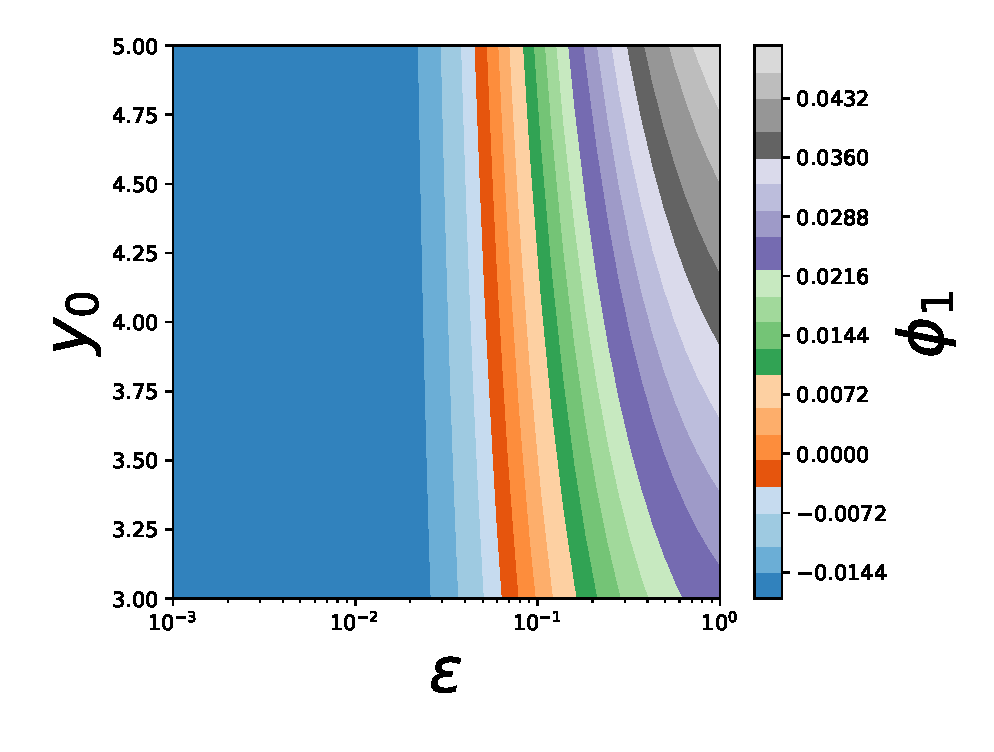
\includegraphics[width=0.33\textwidth]{y0_eps_phi1_sing} &
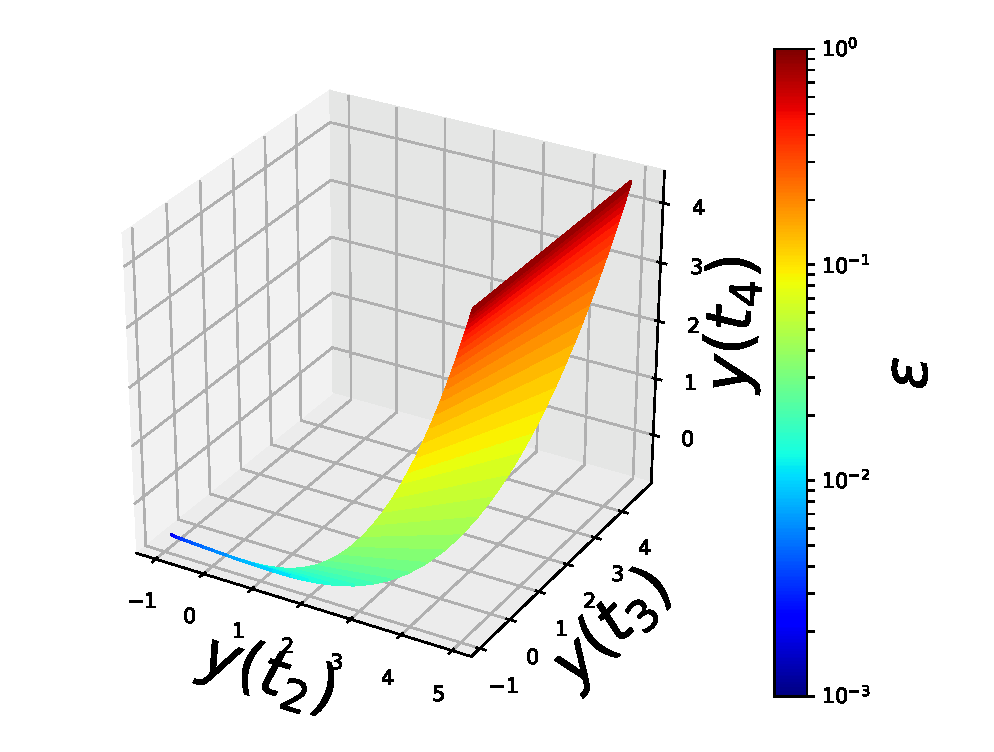
\includegraphics[width=0.33\textwidth]{mod_man_epsilon} &
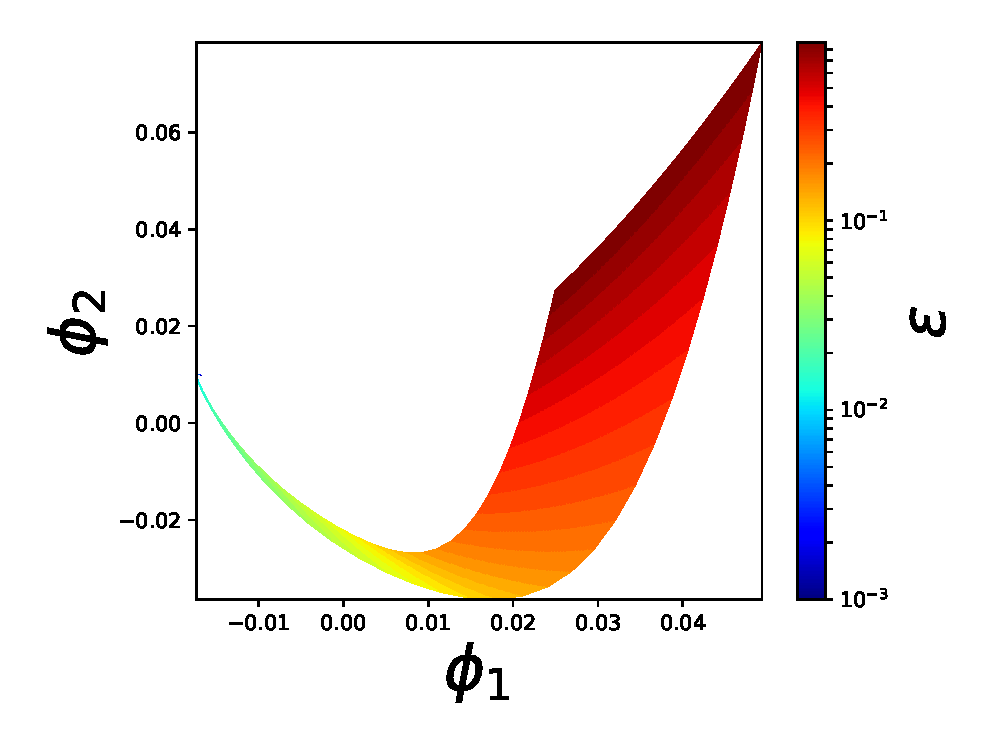
\includegraphics[width=0.33\textwidth]{phi2_phi1_eps_sing} \\
(a) & (b) & (c)\\
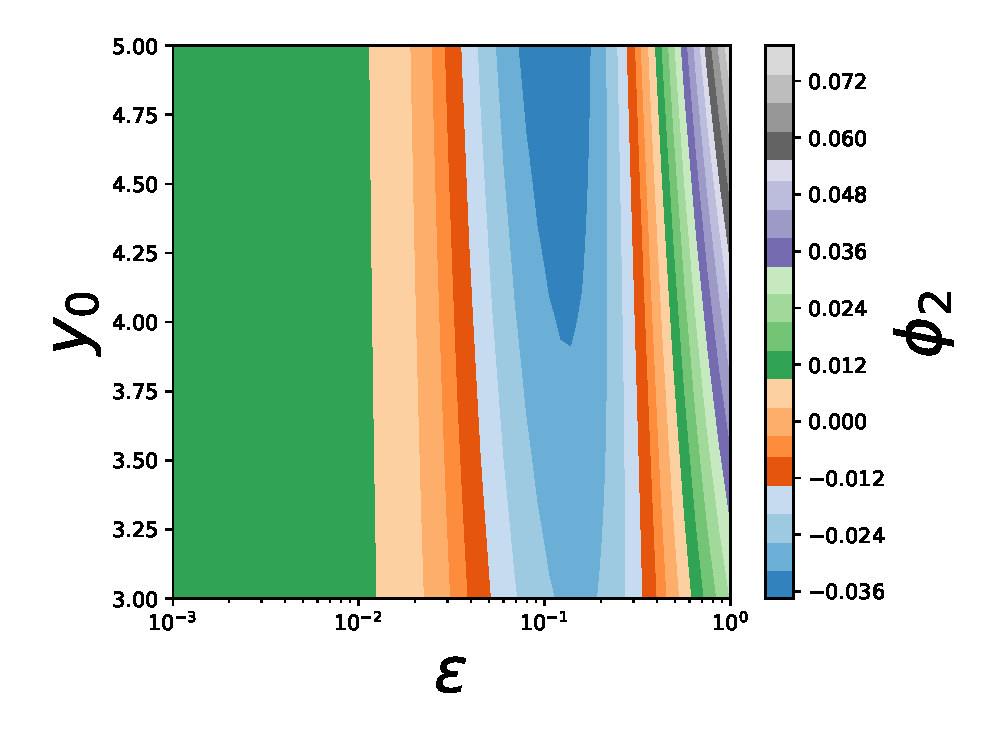
\includegraphics[width=0.33\textwidth]{y0_eps_phi2_sing} &
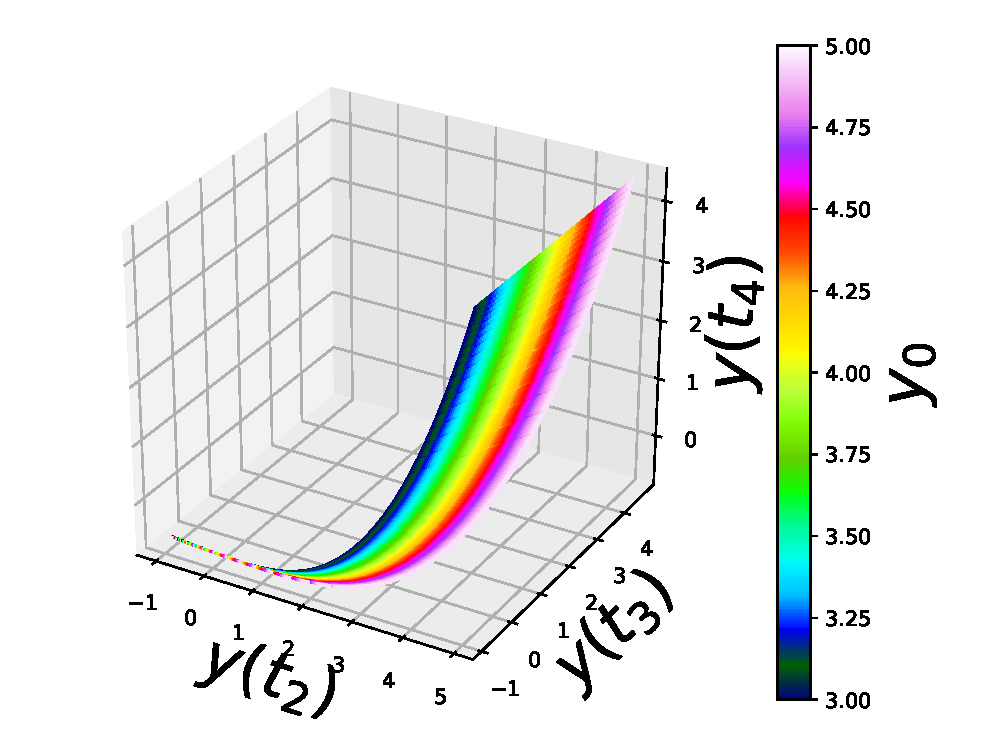
\includegraphics[width=0.33\textwidth]{mod_man_y0} &
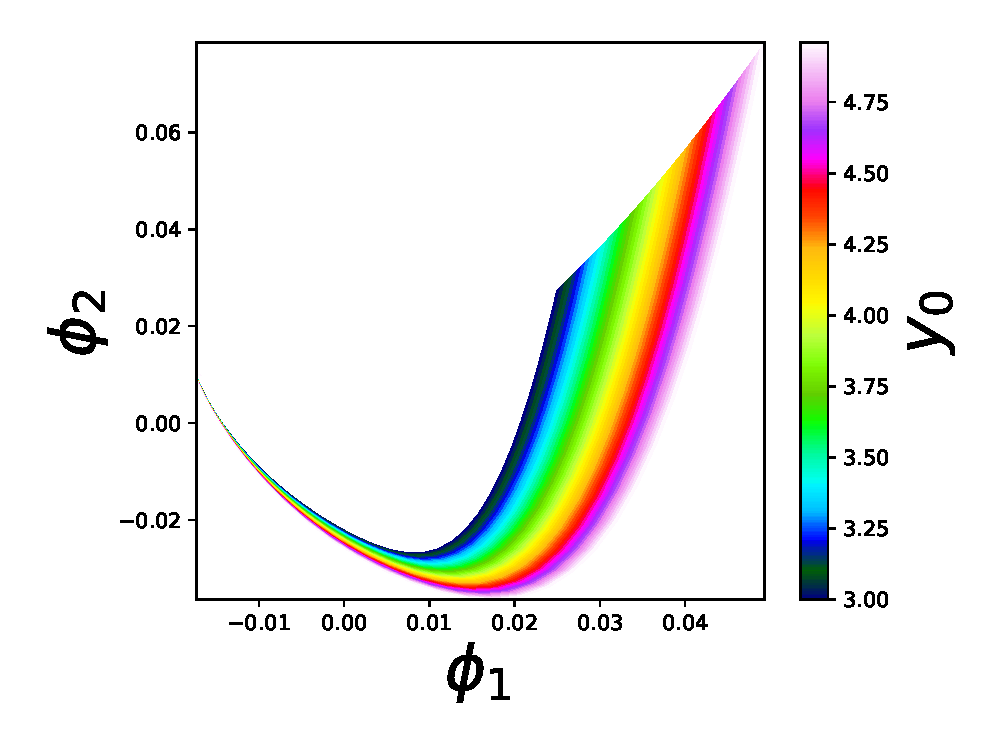
\includegraphics[width=0.33\textwidth]{phi2_phi1_y0_sing}  \\
(d) & (e) & (f)\\
\end{tabular}
\caption{(a) \& (d) Parameter space colored by $\phi_1$ and $\phi_2$;
  (b) \& (e) Model manifold colored by $\epsilon$ and $y_0$; (c) \&
  (f) Diffusion map space colored by $\epsilon$ and
  $y_0$ \label{fig:singpert-dmaps}}
\end{figure}


\begin{figure}[!htp]
\centering
\begin{tabular}{c}
\includegraphics[height=0.3\textheight]{y0-eps-patches} \\
(a)\\
\includegraphics[height=0.3\textheight]{y4-y3-y2-patches}\\
(b)\\
\includegraphics[height=0.3\textheight]{phi2-phi1-patches}\\
(c)\\
\end{tabular}
\caption{(a) Patches in parameter space for singularly perturbed
  system; (b) Patches in model response space for singularly perturbed
  system; (c) Patches in DMAPS embedding space for singularly
  perturbed system \label{fig:singpert-patches}}
\end{figure}


\section{Discussion}




% By modifying the traditional DMAPS kernel to bias our random walks
% along sloppy directions in parameter space, we have developed an
% automated method of uncovering nonlinear effective parameters in
% complex models. Future work will focus on using these embeddings to
% accelerate optimization in these settings, where simple gradient
% descent based techniques often become trapped in sloppy regions of
% parameter space and converge slowly.

% \section{Sloppiness in parameters and initial conditions}

% To fix ideas and definitions, we start with a dynamical model
% % 
% \begin{equation}
%   \dot{\mathbf{x}}(t \vert \theta)
%   =
%   \mathbf{v}(\mathbf{x} \vert \theta) ,
%   \ \mbox{where} \
%   \dot{\mathbf{x}}
%   =
%   \frac{d\mathbf{x}}{dt}
%   \ \mbox{and} \
%   \mathbf{x}(t_0 \vert \theta) = \mathbf{x}_0(\theta) .
%   \label{x'=v}
% \end{equation}
% % 
% The vector $\mathbf{x}(t \vert \theta) \in \mathbb{R}^d$ collects
% the state variables, also called just "variables", at time $t$ that
% correspond to the vector field
% $\mathbf{v} : \mathbb{R}^d \times \mathbb{R}^M \to \mathbb{R}^d$, to
% the parameter settings $\theta \in \mathbb{R}^M$ and to the
% initial state $\mathbf{x}_0(\theta)$.  The \emph{output} of
% \eqref{x'=v} is the system state $\mathbf{x}(t \vert \theta)$ for
% all times $t>t_0$, written $\mathbf{x}(\cdot\vert\theta)$, but
% \emph{data} are only partial observations of that time course.
% Observing the system means recording a number $N \ge M$ of outputs
% into an $N-$tuple $f(\theta) \in \mathbb{R}^N$, for fixed
% settings $\theta$.  Each setting $\theta$ yields a
% well-defined \emph{model response} $f(\theta)$ and, as
% $\theta$ moves in parameter space, $f(\theta)$ traces
% out a (generically $M-$dimensional) output manifold $\mathcal{M}$ in
% data space $\mathbb{R}^N$.  We will be writing
% $\mathcal{M}-$\emph{manifold} to conform with the ``model manifold''
% term in \cite{TMS}.

% % By observation we understand \emph{quantification} through a set of
% % measurement functions $f_1,\ldots,f_N$ transforming the time course
% % into numbers, so that data have the form
% %% 
% % \begin{equation}
% %   f(\theta)
% % %   =
% % %   \big[
% %   f_1(\mathbf{x}(\cdot\vert\theta)) \, ,
% % %   \ldots \, ,
% %   f_N(\mathbf{x}(\cdot\vert\theta))
% % %   \big]
% % %   \in
% %   \mathbb{R}^N .
% %   \label{f(x)}
% % \end{equation}
% %% 
% % This maps parameter values $\theta$ to a point in data space
% % $\mathbb{R}^N$ through the mediation of the time course
% % $\mathbf{x}$.  across a domain in $\mathbb{R}^M$

% Fig.~\ref{fig:sing-pert} shows the $\mathcal{M}-$\emph{manifold} for
% the prototypical singularly perturbed model
% % 
% \begin{equation}
%   \dot{x} = -x/\varepsilon, \quad
%   x(0) = x_0 .
%   \label{1D-model-singpert}
% \end{equation}
% For this system, we view both $\varepsilon$ and $x_0$ as parameters
% and monitor $x$ at distinct times $0 < t_1 < t_2 < t_3$, so that
% % 
% \begin{equation}
%   \theta = (\epsilon , x_0)
%   \quad\mbox{and}\quad
%   f(\theta)
%   =
%   \big[
%   x(t_1 \vert \theta) \, ,
%   x(t_2 \vert \theta) \, ,
%   x(t_3 \vert \theta)
%   \big] . 
%   \label{1D-pf}
% \end{equation}
% % 
% % Sliding down $\mathcal{M}$ in the plot amounts to decreasing $\epsilon$
% % and increasing $x_0$.
% In the spirit of the bound-to-bound approach by Frenklach and
% co-workers, it is instructive to compare side by side how boundaries
% on the $\mathcal{M}-$manifold map to parameter space and vice versa.
% Fig.~\ref{fig:sing-pert} shows several nested subdomains of the
% $\mathcal{M}-$manifold created by intersecting that manifold with
% concentric spheres, that is, the domains
% $\|f(\theta) - f(\theta^*)\| \le \delta$
% with $f(\theta^*)$ the center and for various tolerances
% $\delta$.  The smallest, dark blue boundary is fully contained in the
% manifold interior and maps to a compact, ellipse-like subset of
% parameter space: all settings inside it yield responses within the
% smallest tolerance.  That preimage grows with $\delta$ and eventually
% becomes unbounded (light blue boundary) when the subdomain becomes
% tangent to the $f_1-$axis (boundary~B), with the point of
% tangency mapping to infinity on the parameter plane.  Even larger
% boundaries are only partly contained in the $\mathcal{M}-$manifold and
% their preimages also unbounded, with the one tangent boundary~A
% extending to $\varepsilon=0^+$ (orange boundary).

% This manifests that boundaries of the $\mathcal{M}-$manifold
% correspond to asymptotic regimes themselves \cite{TQ}, namely
% $\varepsilon \gg t_3$ for A and $\varepsilon \ll t_1$ for B or, for
% fixed observation times, $\varepsilon \to \infty$ and
% $\varepsilon \to 0$.  As a result,
% $f(\theta) = (x_0,x_0,x_0)$ for $\varepsilon \to \infty$,
% so that boundary~A is parameterized by the initial condition $x_0$
% alone: the model output becomes \emph{sloppy} in $\epsilon$ and
% one-dimensional.  The regime $\varepsilon \to 0$, on the other hand,
% corresponds to a singularly perturbed problem, with boundary~B
% parameterized by
% $x(t_1 \vert \theta) = x_0\mathrm{e}^{-t_1/\varepsilon}$.  In that
% regime, $x(t_1 \vert \theta)$ converges to the origin for finite
% $x_0$, so that our system effectively becomes zero-dimensional.  Had
% such a singular perturbation occurred in the context of a larger
% system of differential equations, we would have been able to reduce
% the number of state variables needed to describe our system.  hence,
% by including initial conditions as model parameters, we can
% effectively find possible reductions in both parameter- and
% state-space.  Another important observation is that the qualitative
% features of the $\mathcal{M}-$manifold are model features, independent
% of parameter inference and fitting (subdomains) and relating to
% working in the vicinity of an $\mathcal{M}-$manifold boundary.
% Clearly, grouping different system outputs into $f$ would
% give α different $\mathcal{M}-$manifold.

% \begin{figure*}
%   \centering
%   \begin{subfigure}[t]{0.45\linewidth}
%     \centering
%     \includegraphics[height=2in]{f3-f2-f1-delta-cropped}
%     \subcaption{Model manifold with overlaid contour lines for
%       $\delta$ equal to $0.01$, $0.06$, $0.10$, $0.14$, $0.22$, $0.28$
%       and $0.34$.  Boundary~A ($f_1 = f_2 = f_3$) marks the regime
%       $\epsilon \rightarrow \infty$ and boundary~B ($f_2 = f_3 = 0$)
%       the regime $\epsilon \rightarrow0$.
%       \label{fig:sing-pert-mm} }
%   \end{subfigure}
%   \hspace{0.5cm}
%   \begin{subfigure}[t]{0.45\linewidth}
%     \centering
%     \includegraphics[width=1.0\linewidth]{x0-eps-delta-singpert}
%     \subcaption{Parameter space of the singularly perturbed system
%       with contour lines from left figure for $\delta$ equal to
%       $0.01$, $0.06, 0.10, 0.14, 0.22, 0.28, 0.34)$. At the light blue
%       curve which intersects the $f_1$ axis, the curve opens up to the
%       right as $\epsilon \rightarrow 0$, while at the light red curve
%       which intersects the $f_1 = f_2 = f_3$ line, the contour also
%       opens up towards the left as $\epsilon \rightarrow
%       \infty$. \label{fig:sing-pert-params} }
%   \end{subfigure}
%   \caption[Model manifold and parameter space of the singularly
%     perturbed system]{Model manifold and parameter space of the singularly
%     perturbed system \eqref{1D-model-singpert} with select $\delta$
%     contours.
%     \label{fig:sing-pert} }
% \end{figure*}
% % 

% We conclude this section by contrasting regular to singular
% perturbations through the equally simple model
% % 
% \begin{equation}
%   \dot{x} = -\epsilon x^3 - x,
%   \quad
%   x(0) = x_0 ,
%   \label{1D-model-regpert}
% \end{equation}
% % 
% with $\theta$ and $f$ as above.  Fig.~\ref{fig:reg-pert}
% shows the model manifold and the parameter plane, with the plotted
% contours bounding regions of increasing $\delta$.  These countours
% extend to $\varepsilon = 0^+$ past a certain $\delta$, illustrating
% that the model becomes sloppy for small $\epsilon$ but retains its strong
% dependence on $x_0$.  In regular perturbations, loss of parameters
% occurs without concomitant loss of variables: the model parameters can
% be simplified but the number of variables cannot be reduced.

% \begin{figure*}
%   \centering
%   \begin{subfigure}[t]{0.45\linewidth}
%     \centering
%     \includegraphics[width=\linewidth]{x3-x2-x1-eps}
%     \caption{Model manifold of regularly perturbed system with
%       parameters $x_0$ and $\epsilon$, colored by $\epsilon$. As
%       $\epsilon$ decreases, the model response is increasingly
%       determined solely by $x_0$ as the system converges to
%       $x' = x^3$. \label{fig:reg-pert} }
%   \end{subfigure}
%   \hspace{0.5cm}
%   \begin{subfigure}[t]{0.45\linewidth}
%     \centering
%     \includegraphics[width=\linewidth]{x0-eps-delta}
%     \subcaption{Parameter plane of the regular perturbation system
%       colored by $\delta^2$, the distance from the base parameter
%       values at $x_0^*$ and $\epsilon^*$. For larger $\epsilon$ both
%       $\epsilon$ and $x_0$ affect the value of $\delta$, while
%       $\delta$ flattens horizontally along the $\epsilon$ axis at
%       small $\epsilon$, only varying in the one remaining important
%       parameter direction: $x_0$. \label{fig:reg-pert-params} }
%   \end{subfigure}
%   \caption[Model manifold and parameter space of the regularly
%   perturbed system]{Model manifold and parameter space of the
%     regularly perturbed system \eqref{1D-model-regpert} with select
%     $\delta$ contours \label{fig:reg-pert} }
% \end{figure*}

% \begin{figure*}[ht!]
%   \centering
%   \includegraphics[width=\textwidth]{mm-combined}
%   \caption[Quantitative illustration of mapping from parameter space
%   to the model manifold]{Correspondence between parameter space (left)
%     and the model manifold (right). At large values of $\epsilon$,
%     rectangles in parameter space are mapped to skewed rectangles on
%     the model manifold. At intermediate values of $\epsilon$, they are
%     stretched into nearly one-dimensional segments. At small values
%     where the system is singularly perturbed, patches in parameter
%     space map to approximately the same point on the model manifold,
%     the hallmark of sloppiness.}
% \end{figure*}

% \section{Parameter inference}

% Parameter sloppiness builds on the observation that different
% parameter perturbations can affect the generated data drastically
% differently, despite the existence of a one-to-one correspondence
% between data and parameters.  This is already reflected in eigenvalue
% disparities in an SVD of the Jacobian
% $D_\thetaf(\theta)$, with small eigenvalues tied to
% \emph{sloppy parameter directions} that hardly affect the data.
% Although Jacobian-based sensitivity analysis is local, the footprint
% of sloppiness is the existence of \emph{extended} regions in parameter
% space evoking nearly identical data.  Such neutral sets are
% effectively lower-dimensional and roughly foliate full-dimensional
% regions of parameter space, with effective system parameters remaining
% approximately constant on them.

% % Finally, we note that sloppiness is an open property of the input--output system characterizing entire regimes in input space and often linked with manifold boundaries.\\

% In the context of the perturbed model corresponding to
% Fig.~\ref{fig:non-id}, an $M-$dimensional ball around
% $f^*=(1,0,1)$ is pulled back to an ellipsoid centered at
% $\theta = (1,1)$ with widely disparate principal axes.  The
% largest principal directions correspond to sloppy parameter
% combinations, and they can be unraveled by linear algebraic techniques
% such as Principal Component Analysis.  In reality, pronounced
% deviations of \eqref{1D-model-singpert} from linearity mean that
% neighborhoods of $f^*$ are mapped to curved neutral sets in
% parameter space with disparate characteristic length scales; this is
% already evident in Fig.~\ref{fig:sing-pert}.  Such neutral sets are
% not directly amenable to linear techniques, requiring instead the
% development of a nonlinear data mining framework to identify them and
% the associated effective parameters.  We will make these ideas
% concrete below through a series of examples.

% \section{Visualizing nonlinear sloppiness}
% The classical technique to analyze parameter sensitivity is through
% analysis of the singular values of the Jacobian
% $D_\thetaf(\theta)$.  Large disparities suggest
% directions in parameter space along which the model response
% $f$ remains essentially constant.  Due to its local nature,
% this technique fails to uncover parameter sloppiness or yields
% misleading results if there are strong nonlinearities present in the
% effective parameter set. We review a few illustrative examples
% directly below.

% \subsection{Creating sloppiness} \label{sec:hm} Consider a
% prototypical nonlinear ODE model crafted from the linear system

% \begin{align}
%   \begin{aligned}
%     X' &= -\lambda X , \\
%     \epsilon Y' &= -Y ,
%     \label{eqn:sp}
%   \end{aligned}
% \end{align}

% by passing to new state space coordinates given implicitly by
% $(X, Y) = (x-\beta y^2 , y - \alpha x^2)$.  The result is a nonlinear
% but tractable ODE model with parameters
% $\alpha,\beta,\lambda,\epsilon$.  For reasons of illustration, we set
% $\theta = (\alpha,\lambda)$, keeping $\beta$ and $\epsilon$ fixed at
% $10^{-2} and 10^{-3}$ with $\epsilon \ll \lambda$.  In that regime,
% the ODE system is singularly perturbed with a slow manifold
% $y = a x^2$ that attracts each initial conditions $(x_0,y_0)$ in a
% neighborhood of the origin along the fast fiber
% $x = b y^2 + x_0 - b y_0^2$.  We set the model response to
% \begin{align}
%   f^*(\theta) = \begin{bmatrix} x(t_1;\theta) , \cdots , x(t_{N};\theta) , y(t_1;\theta) , \cdots , y(t_{N};\theta) \end{bmatrix}^\mathrm{T} ,
% \end{align}
% for some number $N=5$ and times evenly spaced in $t \in [0.5, 2.5]$.
% The parameters $\alpha$ and $\lambda$ control the curvature of and
% slow decay on the slow manifold, and neither is sloppy
% (Fig.~\ref{fig:henon}, right panel).  The situation might nevertheless
% appear entirely different once transformed parameters are introduced.
% Using the contrived but illustrative map
% $\theta = (u_4(\alpha,\lambda), w_4(\alpha,\lambda)$, where
% $(u_4,w_4)$ is the fourth iteration of the H\'{e}non map
% \begin{align}
%   \begin{aligned}
%     u_{n+1} &= 1 - \gamma u_n^2 + w_n , \\
%     w_{n+1} &= \zeta u_n ,
%     \label{eqn:henon}
%   \end{aligned}
% \end{align}
% yields a new parameter set that is in one-to-one correspondence with
% the original one but highly nonlinear.  Sloppiness is here pronounced
% (Fig.~\ref{fig:henon}, left panel), with the neutral set being
% elongated, bent and folded.  Again, we stress that one cannot know
% \textit{a priori} the structure of the parameter space.  All one has
% is two ``knobs'' tuning the system, and the existence of the parameter
% set $(\alpha,\lambda)$ is not known in advance.

% To investigate the structure of the neutral sets corresponding to some
% reference model response $f^*$, we sampled $\theta$
% uniformly on the rectangle $(-2, 30) \times (-1.5, 0.7)$, recording
% for each sample the response $f(\theta)$ it generates and
% the associated squared Euclidean distance
% $\delta(\theta) = \| f(\theta) - f^* \|^2$
% from the reference response $f^*$.  In the absence of noise,
% i.e. for perfect measurements $f(\theta)$, $\delta$ has a
% unique minimum at $\theta^*$.  Fig.~\ref{fig:henon} shows the
% sampled values that yield $\delta<0.4$, colored by their
% $\delta-$value, both in $\theta-$ and in $(\alpha,\lambda)-$space.
% The nonlinear character of the model is evident in the deviation of
% the neutral set from an elliptical shape, mild in the
% $(\alpha,\lambda)-$space and overpronounced in $\theta-$space.

% The significance of this example is twofold.  First, parameter
% sloppiness may be accompanied by nonlinearities in the underlying
% model that invalidate traditional sensitivity analysis.  Second, we
% see that this phenomenon is really a result of a poorly parameterized
% model, which an appropriate re-parameterization can largely
% ameliorate.  This suggests two approaches to address model sloppiness:
% develop techniques capable of handling nonlinearity and work with the
% original, nonlinear model, or develop techniques to directly remove
% the nonlinearity from the model.  This paper takes the former
% approach.

% \begin{figure*}[ht!]
%   \centering
%   \includegraphics[width=\textwidth]{p2-p1-delta-l-a-delta}
%   \caption[H\'{e}non map transformed parameters and original
%   parameters in nonlinear singularly perturbed system]{Parameter space colored by $\delta$; all points satisfy $\delta<0.4$. H\'{e}non map transformed parameters $w_4$ and $u_4$ (left), and original parameters $\alpha$ and $\lambda$ (right). Here, we used the classical values  $(\gamma,\zeta) = (1.4,0.3)$ for the H\'{e}non map. The central point at $\delta=0$ corresponds to $(\lambda^*, a^*) = (1, 1)$.
%     % $\theta^* = (0.7956, 1.8)$
%     \label{fig:henon} }
% \end{figure*}




%%% Local Variables: ***
%%% mode:latex ***
%%% TeX-master: "../../thesis.tex"  ***
%%% End: ***